% !TEX root = ../Poissons.tex




\subsubsection{The Diagonals}

\begin{definition}
Let $D(n) := \{ \{I,J\}:I,J \subset \{1,\dots,n\}, |I|= |J|, I\cap J = \emptyset \}$.
This is a set of unordered pairs, however there are two clear ways to order these pairs. We say $I<J \equiv (I,J)$ if,
\begin{itemize}
    \item $LA : \min(I\cup J) = \min I$
    \item $SU : \max(I\cup J) = \max J $
\end{itemize}
and we will denote $D(n)$ ordered in one of these two fashions as $LA(n)$ and $SU(n)$.
Our naming convention arises as the $LA$ order induces the $\OP^{LA}$ diagonal (through \cite[Theorem 3.16]{LA21}) and we will show in ... that the $SU$ order induces the $\OP^{SU}$ diagonal.
We will also use $-^{op}$ to refer to the dual of these orders. We say an $\{I,J\}$ pair is of order $k$ if $|I| = |J|=k$. 
\end{definition}

\begin{definition}
We say an ordering of $D(n)$ is \emph{coherent} if for all ordered $(I,J)$ pairs 
\begin{align*}
    (I,J) = (\bigsqcup_{a\in A} I_a, \bigsqcup_{a \in A} J_a) \iff \forall a \in A, r((I_a, J_a))
\end{align*}
where $\bigsqcup_{a\in A} I_a$ and $\bigsqcup_{a \in A} J_a$ are partitions of $I,J$ using a common indexing set $A$. Each $(I_a,J_a)$ is an ordered pair of $D(n)$, and $r$ is the standardisation function e.g. $r( (\{5,9,10\},\{6,8,12\})) = (\{1,4,5\},\{2,3,6\})$.
\end{definition}

\begin{lemma} \label{coherent lemma}
The $LA$ and $SU$ orderings are coherent, and are coherent extensions of the following $(I,J)$ pairs,
\begin{itemize}
    \item ${LA} :$ for all $k\geq 1$  $(\{1,k+2,k+3,\dots,2k-1,2k\}, \{2,3,\dots,k+1\})$
    \item ${SU} :$ for all $k\geq 1$  $(\{k,k+1,\dots,2k-1\},\{1,2,3,\dots,k-1,2k\})$
\end{itemize}
The dual orders $LA^{op}$ and $SU^{op}$ are also coherent, and coherent extensions of the dual pairs.
\end{lemma}

\begin{proof}
We present the proof for ${LA}$, the proof for ${SU}$ proceeds similarly, and the dual proofs are obtained from duality.
Let $o_k:= (I_k,J_k):= (\{1,k+2,k+3,\dots,2k-1,2k\}, \{2,3,\dots,k+1\})$. It is apparent that $o_k$ is not a union of other $I,J$ pairs as $1$ is the only element of $I_k$ which is smaller than other elements of $J_k$.
As such, if we tried to decompose it as a union we could pick out one pair $(I_1,J_1)$ such that $\min ( I_1\cup J_1) = \min I_1 = 1$, but the next possible pair must satisfy $\min ( I_2\cup J_2) = \min J_2$, and hence would violate the $LA$ order.
\\\\
For any other $(I,J)$ pair of order $k$ which does not reduce to $o_k$, there exists $i_2 \in I\setminus \min I$ such that $i_2 < \max J$.
This means every other pair can be decomposed as a union. In particular, if our pair is such that $r(I,J)=(\{i_1,\dots,i_k\},\{j_1,\dots,j_k\})$ (each set ordered smallest to largest), then it must be the case that $1=i_1<i_2<j_k$.
In which case, $(\{i_2\},\{j_k\})$ and $(\{i_1,i_3,\dots,i_k\},\{j_1,\dots,j_{k-1}\})$ are both smaller $(I,J)$ pairs.
We note that there are potentially other ways to decompose an $(I,J)$ pair. 
However, if $(I,J) = (\sqcup_{a\in A} I_a, \sqcup_{a \in A} J_a)$, then the ${LA}$ order is such that $\forall a \in A, r((I_a, J_a))$.
As such all decompositions of a pair $(I,J)$ order it the same way.
\\\\
Finally, we show that $LA$ is a coherent extension of the $o_k$.
Suppose we decompose $(I,J)$ into $(\{i_2\},\{j_k\})$ and $(\{i_1,i_3,\dots,i_k\},\{j_1,\dots,j_{k-1}\})$.
Then it must be the case that $r((\{i_2\},\{j_k\})) = (\{1\},\{2\})$, and $r((\{i_1,i_3,\dots,i_k\},\{j_1,\dots,j_{k-1}\}))$ is either $o_{k-1}$ or we can repeat this decomposition.
This repeated decomposition must eventually terminate with the RHS reducing to $o_{l}$ for $1 \leq l \leq k-1$.
Consequently, any $(I,J) = (\{i_1,...,i_k], \{j_1,...,j_k\})$ decomposes as
\begin{align*}
	(I,J) = (\{i_2\},\{j_k\}) \cup (\{i_3\},\{j_{k-1}\}) \cup ... \cup (\{i_{l+1} \},\{j_{k-l-1} \}) \cup (I'_l,J'_l)
\end{align*}
where $r((I'_l,J'_l)) = o_l$, and $1\leq l \leq k$.
\end{proof}

\begin{lemma}
The only coherent orderings of $D(n)$ are $LA,SU,LA^{op}$ and $SU^{op}$.
\end{lemma}

\begin{proof}
We first observe that there are precisely $4$ ways to order the $D(n)$ pairs of size $k\leq 2$ such that the coherent extension of these orders do not collide.
These are,
\begin{enumerate}
    \item $(\{1\},\{2\})$ and $(\{1,4\},\{2,3\})$ which corresponds to $\OP$ i.e. $\min(I\cup J) = \min I$
    \item $(\{1\},\{2\})$ and $(\{2,3\},\{1,4\})$ which corresponds to $SU$ i.e. $\max(I\cup J) = \max J$
    \item $(\{2\},\{1\})$ and $(\{2,3\},\{1,4\})$ which corresponds to $\OP^{op}$ i.e. $\min(I\cup J) = \min J$
    \item $(\{2\},\{1\})$ and $(\{1,4\},\{2,3\})$ which corresponds to $SU^{op}$ i.e. $\max(I\cup J) = \max I$
\end{enumerate}
More specifically, we must order the sole reduced $D(n)$ pair of order $1$, $\{\{1\},\{2\}\}$.
Then once we have ordered this pair, the sole reduced $D(n)$ pair of order $2$ which must be ordered is $\{\{1,4\},\{2,3\} \}$.
There are clearly $4$ ways to order these two pairs, and we can identify these $I,J$ pairs as cases of \cref{coherent lemma}.
\\\\
We now show that once we have committed to one of these four orders we must follow through with it.
We will show this through induction for the $LA$ order, the $SU$ order proceeds similarly, and the dual orders by duality.
\\\\
Let $l\geq 2$ and suppose that $\forall k\leq l$ that $\{1,k+2,k+3,\dots,2k-1,2k\} < \{2,3,\dots,k+1\} $.
Then from \cref{coherent lemma} we know that the only $\{I,J\}$ pair of order $l+1$ that will not decompose (and hence be specified by admissibility) is 
$$\{\{1,(l+1)+2,(l+1)+3,\dots,(l+1)k-1,2(l+1)\}, \{2,3,\dots,(l+1)+1\}\}$$
As such, the only way we can vary from $LA$ is to order this element in the opposite direction i.e.
$$\{2,3,\dots,(l+1)+1\} < \{1,(l+1)+2,(l+1)+3,\dots,(l+1)k-1,2(l+1)\} $$
However, if we make this choice than this leads to contradictions in the ordering of the $\{I,J\}$ pairs of order $l+2$.
The following contradiction is a generalisation of \cref{ex:Non-coherent order contradiction}.
Let $m = l+2$, then the pair
$$\{I,J\}:= \{ \{1,3,m+3,m+4,\dots,2m-1,2m\}, \{2,4,5,\dots,m+2\} \}$$
can be oriented in both directions.
In particular $\{I,J\} = \{I_1 \cup I_2, J_1 \cup J_2\} = \{I'_1 \cup I'_2, J'_1 \cup J'_2\}$ where
\begin{align*}
    I_1:= \{1,m+3,\dots,2m\} > J_1:= \{4,5,\dots,m+2\} \text{ and } I_2:=\{3\} > J_2:= \{2\}
\end{align*}
this decomposition makes use of the (reversed) order $l+1$ case and the (non-reversed) order $1$ case.
The second decomposition,
\begin{align*}
    I'_2:= \{1,m+3,\dots,  2m-1\} < J'_1:= \{2,5,\dots,m+1\} \text{ and } I'_2:=\{3, 2m\} < J'_2:= \{4, m+2\}
\end{align*}
makes use of the (non-reversed) order $l$ and $2$ cases.
\end{proof}

\begin{example} \label{ex:Non-coherent order contradiction}
Suppose the $LA$ order holds for $D(n)$ of order $k\leq 2$ and in order $3$ it is reversed, i.e.
\begin{align*}
    \{1\}<\{2\},\quad \{1,4\}< \{2,3\}, \quad \{2, 3, 4\} < \{1, 5, 6 \}
\end{align*}
Then $\{I,J\}=\{\{1, 3, 7, 8\}, \{2, 4, 5, 6\}\}$ admits two different orientations.
In particular, 
\begin{align*}
    \{1, 7, 8\} > \{ 4, 5, 6 \} \text{ and } \{3\} > \{2\} &\implies \{1, 3, 7, 8\} >\{2, 4, 5, 6\}\\
    \{1, 7\}< \{2, 5\} \text{ and } \{3, 8\}< \{4, 6\} &\implies \{1, 3, 7, 8\} <\{2, 4, 5, 6\}
\end{align*}

\end{example}

As a consequence of these lemmas and Theorem 3.16 of \cite{LA21} \Kurt{and tree substitution...}it follows that, 
\begin{thm}
There are only four comultiplicative diagonals of every operahedra, in particular, those induced by the $LA, SU, LA^{op}$ and $SU^{op}$ orders on $D(n)$.
\end{thm}

There are four clear bijective maps between these four orders of $D(n)$
\begin{center}
\begin{tikzcd}
\OP \arrow[r,"s"] \arrow[d,"i"]&
\OP^{op}\arrow[d,"i"]\\
SU^{op} \arrow[r,"s"] &
SU
\end{tikzcd}
\end{center}
where $s(I,J):=(J,I)$ and $i$ inverts the order on an $(I,J)$ pair, mapping the smallest element to the largest element, then the next smallest to next largest and so on, e.g. 
\begin{align*}
    i(\{1, 7, 8\} , \{ 4, 5, 6 \}) = (\{8,2,1\},\{7,6,5\}) = (\{1,2,8\},\{5,6,7\})
\end{align*}
These bijections in orders induce a bijection between the diagonals. 
\begin{proposition}
There is a bijection between diagonals $\theta:\OP^{LA} \to \OP^{SU}$.
\end{proposition}
\begin{proof}
For any pair $(\sigma,\tau)$ of ordered partitions of $[n]$, we have
\begin{align*}
    (\sigma,\tau)\in \OP^{LA}
    \iff  \forall (I,J) \in LA(n), &\exists k, \bigg| \bigcup_{i=1}^k \sigma_i \cap I \bigg| > \bigg|\bigcup_{1=1}^k \sigma_i \cap J \bigg|
    \\
    \text{ or } 
    &\exists l, \bigg| \bigcup_{i=1}^l \tau_k \cap I \bigg| < \bigg|\bigcup_{i=1}^l \tau_l \cap J \bigg|
\end{align*}
and \Kurt{Here negative indexing is indexing in reverse. This really cleans up notation. }
\begin{align*}
    (\sigma,\tau)\in \OP^{SU}
    \iff  \forall (I,J) \in SU(n),
    &\exists k, \bigg| \bigcup_{i=1}^{k} \tau_{-i} \cap J \bigg| > \bigg|\bigcup_{i=1}^{k}\tau_{-i} \cap I \bigg|
    \\
    \text{ or } 
    &\exists l, \bigg| \bigcup_{i=1}^{l} \sigma_{-i} \cap J \bigg| < \bigg|\bigcup_{i=1}^{l} \sigma_{-i} \cap I \bigg|    
\end{align*}
Let $\theta ((\sigma,\tau)) := (\overline{\tau},\overline{\sigma})$, where an ordered $[n]$ partition $\sigma_1|...|\sigma_k$ is mapped to $\overline{\sigma}:=\overline{\sigma_{k}} | \ldots | \overline{\sigma_{1}}$, where $\overline{\sigma_i}$ is the set $\{n-j+1 \ | \ j \in \sigma_i\}$. In words, the $\overline{\sigma}$ reverses the order of the blocks of $\sigma$, and reverses the order of its constituents i.e. $1\mapsto n,2 \mapsto n-1,...,n\mapsto 1$. To see that $\theta$ is well defined, observe that under the bijection between $LA(n)$ and $SU(n)$ that $(I,J) \in LA(n)$ is mapped to $(J',I'):=(i(J),i(I)) \in SU(n)$. As such,
\begin{align*}
    (\sigma,\tau)\in \OP^{LA}
    \iff  \forall (J',I') \in SU(n), 
    &\exists k, \bigg| \bigcup_{i=1}^{k} \sigma'_{-i} \cap I' \bigg| > \bigg|\bigcup_{i=1}^{k} \sigma'_{-i} \cap J' \bigg|
    \\
    \text{ or } 
    &\exists l, \bigg| \bigcup_{i=1}^{l} \tau'_{-i} \cap I' \bigg| < \bigg|\bigcup_{i=1}^{l} \tau'_{-i} \cap J' \bigg|
\end{align*}
i.e. we translate the the $\OP^{LA}$ conditions imposed on $(\sigma,\tau)$ through $\theta$. Hence, by definition $(\tau',\sigma')\in \OP^{LA}$. From here, it is immediate that $\theta$ and its clear inverse are both injective, so we have a bijection.
\end{proof}

Furthermore, this bijection is a face poset isomorphism.  
\begin{lemma}
Given two faces $(\sigma,\tau),(\sigma',\tau') \in \triangle$, then $(\sigma',\tau')$ is a face of $(\sigma,\tau) $ iff $\mathcal{N}(\sigma,\tau) \subset \mathcal{N}(\sigma',\tau')$. Furthermore, $(\sigma',\tau')$ is a facet of $(\sigma,\tau) $ iff $\mathcal{N}(\sigma,\tau) \subset \mathcal{N}(\sigma',\tau')$ and $|\mathcal{N}(\sigma',\tau')| = |\mathcal{N}(\sigma,\tau)|+1$.
\end{lemma}
\begin{proof}
...
\end{proof}
The bijection between ordered partition (pairs) and (pairs of) nestings may be used to translate this lemma as follows. \Kurt{What is the shortest path to this corollary that uses the least amount of nesting theory?}
\begin{corollary}
Given two faces $(\sigma,\tau),(\sigma',\tau') \in \triangle$ (either $\OP^{LA}$ or $\OP^{SU}$), then
$(\sigma',\tau')$ is a facet of $(\sigma,\tau)$ iff 
\begin{center}
$\sigma = \sigma'$ and $\tau' = ref_{A,B}(\tau)$ or $\tau = \tau'$ and $\sigma' = ref_{A,B}(\sigma)$
\end{center}
where if $\sigma = b_1|...|b_k$ and $b_i$ is partitioned by $A,B$ then
\begin{align*}
    ref_{A,B}(\sigma) &= b_1|...|b_{i-1}|A|B|b_{i+1}|...|b_k
\end{align*}
\end{corollary}

\begin{lemma}
Given two faces $(\sigma,\tau),(\sigma',\tau') \in \OP^{LA}$,
$(\sigma',\tau')$ is a facet of $(\sigma,\tau)$ iff $\theta((\sigma',\tau'))$ is a facet of $\theta((\sigma,\tau))$.
\end{lemma}
\begin{proof}
We prove the case when $\sigma = \sigma'$ and $\tau' = ref_{A,B}(\tau)$, the other case is similar. We directly compute,
\begin{align*}
    \theta( (\sigma,\tau)) &= (\overline{\tau},\overline{\sigma}) = (\overline{b_k}|...|\overline{b_{i+1}}|\overline{b_i}|\overline{b_{i-1}}|...|\overline{b_1},\overline{\sigma})\\
    \theta( (\sigma',\tau')) &= (\overline{\tau'},\overline{\sigma'}) = (\overline{b_k}|...|\overline{b_{i+1}}|\overline{B}|\overline{A}|\overline{b_{i-1}}|...|\overline{b_1},\overline{\sigma})
\end{align*}
and as $\overline{B}\cup\overline{A}=\overline{b_i}$ it follows that $\theta((\sigma',\tau'))$ is a facet of $\theta((\sigma,\tau))$.
\end{proof}
As a face of face can be identified through a chain of facets, an immediate corollary of this lemma is that $\theta$ is an isomorphism of face posets, i.e,
\begin{corollary}
Given two faces $(\sigma,\tau),(\sigma',\tau') \in \OP^{LA}$,
$(\sigma',\tau')$ is a face of $(\sigma,\tau)$ iff $\theta((\sigma',\tau'))$ is a face of $\theta((\sigma,\tau))$. 
\end{corollary}

\subsection{Bijective results for operadic diagonals}
\label{s:vertices}

\subsubsection{Facets}

In this section we establish a bijection between the facets of $\triangle$ and a family of pairs of unordered partitions introduced and enumerated in a series of 3 papers \cite{chen1969computer,chen1971tables,kajitani1982number}. An intermediary bijection to a type of bipartite tree is of particular importance and provides [...].
In particular, we obtain that the number of facets in the image of the diagonal $\triangle_n$ of the $n$-dimensional permutahedron is $2(n+1)^{n-2}$ (\OEIS{A007334}), and more precisely that the pairs of dimensions $(k,n-k)$ are counted by the formula $\frac{1}{k+1}\binom{n+1}{k}(k+1)^{n-k}(n+1-k)^{k}$. 
\Guillaume{OEIS ref?}


\subsubsection{Essential complementary partitions and bipartite trees}
Let us recall some basic definitions and results from the series of papers \cite{chen1969computer,chen1971tables,kajitani1982number}.

\begin{definition}
A set of \emph{distinct representatives} of a partition $\sigma_I$ is a set $M\subset [n]$ such that $\forall i \in I,|\sigma_i \cap M| = 1$.
\end{definition}

\begin{definition}
A pair of partitions $(\sigma_L,\tau_R)$ is said to be \emph{complementary} if there exists $M\subset [n]$ and $m \in M$ such that $M$ and $([n]\setminus M) \cup \{m\}$ are distinct representatives of $\sigma_L$ and $\tau_R$, respectively.
It is furthermore \emph{essential} if there does not exist proper subsets $ L'\subset L$, $R'\subset R$ and $N' \subset [n]$ such that $(\sigma_{L'},\tau_{R'})$ is a complementary partition of $N'$.
\end{definition}
\begin{definition}
A pair of partitions $(\sigma_L,\tau_R)$ is said to be 
\begin{enumerate}
	\item \emph{complimentary}, if $\forall l\in L, r\in R$ we have that $|\sigma_l \cap \tau_r| \leq 1$
	\item \emph{essential}, if there are no proper subsets of $L'\subset L,R'\subset R$ such that $\cup_{l \in L} \sigma_l = \cup_{r \in R'} \tau_r$
\end{enumerate}	

\end{definition}\Kurt{Maybe can immediately switch to  Vincent's variant of def?}

In cases where there is no ambiguity we will drop the subscripts $L,R$.
We shall denote the set of all essential complementary pairs of partitions of $[n]$ by $\EC$.
Let us emphasize that the pairs of partitions of $\EC$ are \emph{unordered}.

\Guillaume{Notations to be uniformized from here}

\begin{example}
For $n=2$, the two essential complementary partitions are $1|2 \times 12$ and $12 \times 1|2$. For $n=3$, the eight essential complementary partitions are
\begin{align*}
	1|2|3 \times 123,\quad 
	123 \times 1|2|3,\quad 
	1|23 \times 13|2,\quad 
	13|2 \times 1|23\\
	1|23 \times 12|3,\quad 
	12|3 \times 1|23,\quad 
	13|2 \times 12|3,\quad 
	12|3 \times 13|2
\end{align*}
For a larger example see \cref{ex:ECbijection}. 
\end{example}

The reader will have observed from this example, that many pairs of partitions are not essential and complementary.
This can be checked directly from the definition, however, a graphical connection which we now introduce provides a simpler interpretation.
A \emph{tree} is a simply connected graph with no cycles. 
A \emph{bipartite graph} is a graph whose vertices are partitioned into two sets such that vertices in one set are only adjacent to vertices in the other.
We say a bipartite graph is \emph{ordered} if one of the sets is considered smaller than the other and we denote the partition $(V_L,V_R)$. 
We say a graph with $n$ edges is \emph{edge labelled} if there exists a bijection between the edges and $\{1,\dots,n\}$.

\begin{proposition} [{\cite[Theorem 3]{kajitani1982number}}] 
\label{EC Graph Bijection}
The set of essential complementary partitions $\EC$ and the set edge labelled bipartite trees $\BT$ are in bijection.
\end{proposition}
\begin{proof}
Informally, given a partition pair $(\sigma,\tau)$, the corresponding graph $G((\sigma,\tau))$ has the subpartitions of each partition as its vertices, and two vertices are connected by an edge if the subpartitions share a common element. By convention we place the vertices of 
For an example of this bijection see \cref{ex:ECbijection}.
\end{proof}

\subsubsection{Bijection with the facets of the diagonal}

In this section we denote by $\OP$ be the set of pairs of ordered partitions of $[n]$ labeling \emph{facets} of the diagonal $\triangle$. \BDO{We should perhaps change the notation for $\OP$. What about $\triangle_f$ or $\triangle_M$ ?}
\Guillaume{I would keep the indices to the minimum}

\begin{thm}
\label{thm:facets}
Facets of the diagonal and essential complementary partitions are in bijection through the inverse functions $u:\OP \to \EC$ and $o:\EC\to \OP$, where
\begin{enumerate}
    \item The function $u$ forgets the order of the ordered partition pair.
    \item The function $o$ uniquely orders an essential complementary partition pair via the minimal $(I,J)$-pairs defining the diagonal. 
\end{enumerate}
\end{thm}
An immediate corollary of this theorem, and an enumeration of labelled bipartite trees first done in \cite{kajitani1982number}, is that there are $2(n+1)^{n-2}$ facets $\OP_n$.
 This enumeration will be refined in the next section.
We shall prove this theorem by establishing the necessary total order, showing that the functions are well defined, and then showing that they are injective.

\begin{lemma} 
\label{l:u-well-defined}
The function $u:\OP \to \EC$ that forgets the order in a pair of partitions is well defined.
\end{lemma}
\begin{proof}
Let $P \in \OP_n$. Then $G(u(P))$ is a graph with $l+r=n+1$ vertices, and $n$ edges. Furthermore, as no vertices can be isolated it must be the case that this graph is a tree. 
It is straightforward to verify that $G(u(P))$ must be labeled bipartite tree, but here is how we may explicitly produce the necessary distinct representatives using an algorithm of \cite[Theorem 2]{kajitani1982number}.

Let $G'$ be a copy of $G(u(P))$. 
While there is a vertex of degree $1$ in $G'$ delete it and add the sole edge of that vertex as a distinct representative of the corresponding partition of that vertex. 
As $G'$ is a tree this process can continue until there is a single edge connecting two vertices of degree $1$. 
This edge specifies the element $p$ of the distinct representatives.
\end{proof}

\begin{construction} 
\label{Order Lemma}
For $P=(\sigma,\tau) = (\bigcup_{l\in L}\sigma_l,\bigcup_{r\in R} \tau_r) \in \EC$ an essential complementary pair, we construct total orders on the blocks of $\sigma$ and $\tau$ in three steps:
\begin{enumerate}
    \item For $\sigma_l,\sigma_{l'} \in \sigma$ considered as vertices in $G(P)$, there exists a unique minimal path of even cardinality $p_{l,l'}$ connecting them.
    We partition $p_{l,l'}=I\cup J$ where $I$ contains the minimal edge, and the path alternates between elements of $I,J$. Likewise, for $\tau_r,\tau_{r'}\in \tau$ there exists a path and decomposition $p_{r,r'} = I\cup J$.
    \item Direct each path so that all $I$ point left to right, and all $J$ point right to left.
    \item We say $\sigma_l< \sigma_{l'}$ (or $\tau_r < \tau_{r'}$) if the path is directed as $\sigma_l \to \sigma_{l'}$ ($\tau_r \to \tau_{r'}$).
\end{enumerate}
\end{construction}

\begin{proof}
We first show our binary relation is well defined before verifying that it defines a total order on $G(P)$ and hence $P$ via the bijection of \cref{EC Graph Bijection}.

As $G(P)$ is a bipartite tree, every vertex is connected, and every path connecting two vertices on the same side must be of even length. 
As $I$ and $J$ partition the path in an alternating fashion i.e. $p=(i_1,j_1,i_2,j_2,..., )$, we can orient the path by forcing $I$ to point left and $J$ to point right. 
This order is clearly total, reflexive (by convention) and anti-symmetric, what remains to be checked is its transitivity. 

Let $p_{ab}$ denote the unique maximal path between two vertices $a$ and $b$ on the left of $G(P)$, that is two blocks of $\sigma$. 
Let $I_{ab}$ denote the set of left-to-right edges in this path, and let $J_{ab}$ denote its complement. 
Then, we have 
\begin{equation}
    \label{eq:order}
    a < b \iff \min(I_{ab}\cup J_{ab})=\min(I_{ab}) \ . 
\end{equation}
Suppose now that $a < b$ and $b < c$.
Since $p_{ac}= (p_{ab} \cup p_{bc}) \setminus (p_{ab} \cap p_{bc})$, we have $$ I_{ac}=(I_{ab}\cup I_{bc}) \setminus (J_{ab} \cup J_{bc}) \text{ and } J_{ac}=(J_{ab}\cup J_{bc}) \setminus (I_{ab} \cup I_{bc}) \ , $$ and from the condition (\ref{eq:order}) above it is clear that $\min(I_{ac}\cup J_{ac})=\min(I_{ac})$, which completes the proof of the transitivity for the total order on $\sigma$. 
The proof for $\tau$ is similar. 
\end{proof}

\begin{example}\label{ex:ECbijection}
We now illustrate the ordering on the essential complementary partition $15|234|6|7 \times 13|2|46|57$. The fact that this is an essential complementary partition is easily visually verified by constructing its bipartite tree, and this tree, on the left, admits the ordering on the right.
\begin{center}
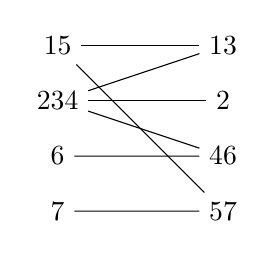
\begin{tikzpicture}[scale=.7]  
\node (1) at (-1.5, -1) {$15$};
\node (2) at (-1.5, -2) {$234$};
\node (3) at (-1.5, -3) {$6$};
\node (4) at (-1.5, -4) {$7$};
%
\node (5) at (1.5, -1) {$13$};
\node (6) at (1.5, -2) {$2$};
\node (7) at (1.5, -3) {$46$};
\node (8) at (1.5, -4) {$57$};
%
\draw[-] (1)--(5); 
\draw[-] (1)--(8);
\draw[-] (2)--(5); 
\draw[-] (2)--(6); 
\draw[-] (2)--(7); 
\draw[-] (3)--(7);
\draw[-] (4)--(8);
%
\end{tikzpicture}
$\quad$
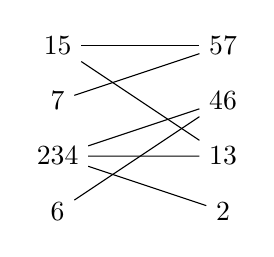
\begin{tikzpicture}[scale=.7]  
\node (1) at (-1.5, -1) {$15$};
\node (2) at (-1.5, -2) {$7$};
\node (3) at (-1.5, -3) {$234$};
\node (4) at (-1.5, -4) {$6$};
%
\node (5) at (1.5, -1) {$57$};
\node (6) at (1.5, -2) {$46$};
\node (7) at (1.5, -3) {$13$};
\node (8) at (1.5, -4) {$2$};
%
\draw[-] (1)--(5); 
\draw[-] (1)--(7);
\draw[-] (2)--(5); 
\draw[-] (3)--(6); 
\draw[-] (3)--(7); 
\draw[-] (3)--(8); 
\draw[-] (4)--(6);
%
\end{tikzpicture}
\end{center}
Here are two examples paths providing order information.
\begin{align*}
	7 <_L 234 \text{ as } 7 \xrightarrow{7} 57 \xrightarrow{5} 15 \xrightarrow{1=I_*} 13 \xrightarrow{3} 234\\
	57 <_R 46 \text{ as } 57 \xrightarrow{5} 15 \xrightarrow{1=I_*} 13 \xrightarrow{3} 234 \xrightarrow{4} 46
\end{align*}
\end{example}


This order far from being arbitrary provides the unique way to order an essential complementary partition pair into an ordered partition pair of $\triangle$, as we shall demonstrate next.

First we need a geometrical lemma. \Kurt{notation clash...}
\begin{proposition}
    The paths between adjacents vertices of $P_L$ or $P_R$ are in bijection with the minimal $(I,J)$-pairs.
\end{proposition}

\begin{proof}
    By \cref{p:minimal-IJ-pairs}, it suffices to show that the paths between adjacent vertices of $P_L$ are in bijection with the solutions of the system of equations of the form $(\rho^1,\sigma^2)$. 
    To ease notation let us write $\rho$ for $\rho^1$ and $\sigma$ for $\sigma^1$. 
    Suppose that $\rho$ is obtained from $\sigma$ by merging the two blocks $\sigma_a$ and $\sigma_b$. 
    The two equations $\langle \vec \sigma_a, x \rangle =0$ and $\langle \vec \sigma_b, x \rangle =0$ now become $\langle \vec \sigma_a + \vec \sigma_b, x \rangle =0$; nothing else changes in the system. 
    Since the solution to the system $(\sigma^1,\sigma^2)$ was $x=0$, now the solution is of dimension $1$, and it is given precisely by the path between $a$ and $b$ in $G(P)$.
    Such a path is given by an alternating sequence of vertices and edges $\sigma_1:=\sigma_a, e_1, \sigma_2, e_2, \ldots, e_{k-1}, \sigma_k:=\sigma_b$. 
    Every edge $e_i \in \{1,\ldots, n\}$ is by definition the intersection $\sigma_{i} \cap \sigma_{i+1}$; thus it is the only common non-zero coordinate between $\vec \sigma_{i}$ and $\vec \sigma_{i+1}$.
    Thus the path encodes the series of equations $x_{e_1}+x_{e_{k-1}}=0$, $x_{e_1}+x_{e_2}=0$, $x_{e_2}+x_{e_3}=0$, $\ldots$, $x_{e_{k-2}}+x_{e_{k-1}}=0$. 
    Thus, $x_{e_1}=1$, $x_{e_2}=-1$, $x_{e_3}=1$, $\ldots$, $x_{e_{k-2}}=1$, $x_{e_{k-1}}=-1$ is a basis of one-dimensional space of solutions, and it gives the corresponding minimal $(I,J)$-pair. 
\end{proof}

\begin{lemma} 
\label{o well defined}
The function $o:\EC \to \OP$ that orders an essential complementary pair is well defined.
\end{lemma}

\begin{proof}
Let $P=(\sigma,\tau) = (\bigcup_{l\in L}\sigma_l,\bigcup_{r\in R} \tau_r) \in \EC$ and consider $o(P)$. 
We first show that every $(I,J)$-condition, for $(I,J) \in D(n)$, which corresponds to a path between vertices is satisfied. 
In particular, this statement will be true for minimal $(I,J)$-pairs, which will be enough in virtue of \cref{p:minimal}. 
Suppose $I,J$ corresponds to a path between two vertices on the left, i.e.
\begin{align*}
    \sigma_l = \sigma_{l_1} \xrightarrow{i_1} \tau_{r_1}\xrightarrow{j_1} \sigma_{l_2} \xrightarrow{i_2}... \xrightarrow{i_{k}} \tau_{r_{k-1}} \xrightarrow{j_k} \sigma_{l_k}= \sigma_{l'}
\end{align*}
By construction we have that $I = \{i_1,...,i_k\},J=\{j_1,...,j_k\} \in D(n)$ (note we are ordering $I$ and $J$ by the path, so it is not necessarily the case that $\min I = i_1$). 
Furthermore, each sub partition of $\tau$ either contains a single element of $I$ and a single element of $J$, or it contains no elements of $I$ and no elements of $J$. 
As such for any ordering of the sub-partitions of $\tau$ we have that \Kurt{Could use [-] notation, but feels clearer to write out?}
\begin{align*}
    \forall m, \bigg|\bigcup_{1\leq k \leq m} \tau_{k} \cap I \bigg| = \bigg|\bigcup_{1\leq k \leq m} \tau_{k} \cap J \bigg|
\end{align*}
Hence in order for this $D(n)$ condition to be satisfied it must be the case that for some ordering of the sub-partitions of $\sigma$ we have
\begin{align*}
    \exists m, \bigg| \bigcup_{1\leq k \leq m} \sigma_k \cap I \bigg| > \bigg|\bigcup_{1\leq k \leq m} \sigma_k \cap J \bigg|
\end{align*}
Every sub-partition of $\sigma$ excluding $\sigma_l$ and $\sigma_{l'}$ either contains no elements of both $I$ and $J$, or it contains a single element of $I$ and a single element of $J$. 
So the only way for the condition to be satisfied is for $\sigma_l$ to come before $\sigma_{l'}$, which is precisely what is required by the total order.

If $I,J$ correspond to a path between two vertices on the right,
\begin{align*}
    \tau_r = \tau_{r_1} \xrightarrow{j_1} \sigma_{l_1}\xrightarrow{i_1} \tau_{r_2} \xrightarrow{j_2}... \xrightarrow{j_{k}} \sigma_{l_{k-1}} \xrightarrow{1_k} \tau_{r_k}=\tau_{r'}
\end{align*}
then a similar chain of logic implies we must have an ordering of the sub-partitions of $\tau$ such that
\begin{align*}
    \exists m, |\bigcup_{1\leq k \leq m}\tau_k \cap I| < |\bigcup_{1\leq k \leq m} \tau_k \cap J|
\end{align*}
and this can only happen if $\tau_r$ comes before $\tau_{r'}$.
\end{proof}

\begin{rem}
    It would be interesting to know if there is a geometrical interpretation of the paths that are not between adjacent vertices. 
\end{rem}

To complete the proof of \cref{thm:facets}, it remains to show that both $u:\OP \to \EC$ and $o:\EC\to \OP$ are injective, with the other function being their inverse.

\begin{proof}[{Proof of \cref{thm:facets}}]
The forgetful function $u$ is clearly the inverse to $o$ as forgetting any assigned order will clearly return the original essential complementary partition pair. 
The ordering function $o$ is the inverse to $u$ as it returns the sole ordering of the sub-partitions which is compatible with the $D(n)$ conditions.
\end{proof}

\Kurt{Quick Corollary of the ordering of SU and an example bijection of facets. Show how paths translate.}

\subsubsection{Vertices}

We are now interested in characterizing the pairs of vertices that occur in the diagonal, that is pairs of permutations $(\sigma_1,\sigma_2) \in \triangle$. 

\begin{thm} There exists $(I,J) \in D(n)$ such that $\forall k, |\sigma_1^1\cdots\sigma_1^k \cap I| \leq |\sigma_1^1\cdots\sigma_1^k \cap J|$ and $\forall l, |\sigma_1^1\cdots\sigma_1^l \cap I| \geq |\sigma_1^1\cdots\sigma_1^l \cap J|$ (diagonal condition) if and only if $\exists (I',J')=(\{i_1,\ldots,i_m\},\{j_1,\ldots,j_m\}) \in D(m)$, $m\leq n$, such that \[\sigma_1 \cap (I'\cup J')=j_1 i_1 j_2 i_2 \cdots j_n i_n \] and \[ \sigma_2 \cap (I'\cup J') = i_2 j_1 i_3 j_2 \cdots i_n j_{n-1} i_1 j_n \ , \] where $i_1 = \min (I' \cup J')$ (fish condition). 
\end{thm}

\begin{proof}
\begin{itemize}
\item If a pair of permutations $(\sigma_1, \sigma_2) \in   \mathfrak{S}_N^2$ satisfies the fish condition, then there exist two sets $I$ and $J$ of same cardinality such that $\min(I)<\min(J)$. Denoting $\sigma_1$ and $\sigma_2$ by two words of size $N$ $\sigma_1^1 \ldots \sigma_1^N$ and $\sigma_2^1 \ldots \sigma_2^N$, then the pair $((\sigma_1, \sigma_2), (I,J))$ satisfies that for any $k$ in $\llbracket 1;N\rrbracket$, $|\sigma_1^1 \ldots \sigma_1^k \cap J| \geq |\sigma_1^1 \ldots \sigma_1^k \cap I|$ and $|\sigma_2^1 \ldots \sigma_2^k \cap I| \geq |\sigma_2^1 \ldots \sigma_2^k \cap J|$, hence the diagonal condition.
\item We will now prove the converse. Let us presume that $(\sigma_1, \sigma_2)$ is a pair of permutations satisfying the diagonal condition for a pair of sets $(I,J) \in D(n)$, minimal for the inclusion of sets.
\begin{description}
\item[Case $n=1$] 
\end{description}
If $|I|=|J|=1$, then it follows directly from the diagonal condition above that ${\sigma_1}_{| I \cup J}=j_1 i_1$ and ${\sigma_1}_{|I \cup J}=i_1 j_1$, hence the fish condition is satisfied.
\begin{description}
\item[Case $n>1$] 
\end{description}
In this case, the proof is made by absurdum 
by considering the number of "well-placed" elements of $I$ and $J$ in $\sigma_1$ and $\sigma_2$. In what follows, for any set $E$, $\sigma^{E}_i$ will stands for $(\sigma_i)_{|E}$. We write also $n_{i,k}^E$ for the number of elements of $E$ in the $k$ first letters of $\sigma_i$. The main argument in each of the small proofs below is the same: if the permutations do not satisfy the pattern described above, then it is possible to find an appropriate pair of elements $(i,j)\in I \times J$ such that $(I-i,J-j)$ satisfies the diagonal condition, hence  contradicting the minimality of $(I,J)$.

We first prove that the leftmost element of $\sigma^{I}_1$ is $i_1$. Indeed, if it is not the case, we consider $i$, the leftmost element in $\sigma^{I}_1$ and $j$ the leftmost element in $\sigma^{J}_2$. The pair $(I-i,J-j)$ is in $D(n-1)$, as $i$ is different from $i_1$. Moreover, it is clear that the diagonal condition still holds for $((\sigma_1, \sigma_2), (I,J))$. As this would contradict the minimality of $(I,J)$, the leftmost element of $\sigma^{I}_1$ is $i_1$.

We then prove that $\sigma^{I \cup J}_1$ starts by $j_1 i_1$ and that this $j_1$ is exactly the leftmost element in  $\sigma^{J}_2$. On that purpose, we suppose that either  $i_1$ is preceeded by several elements of $J$ or that the unique element of $J$ is not the leftmost one in $\sigma^{J}_2$. We then adapt the previous argument by choosing $i$ to be the leftmost element in $\sigma^{I-\{i_1\}}_1$ and $j$ the leftmost element in $\sigma^{J}_2$. The pair $(I-i,J-j)$ is in $D(n-1)$. Let us briefly explain while  the diagonal condition would still be fulfilled in this case. If $j$ is after $i_1$ in $\sigma_1$, then the difference $n_{1,k}^{J-j}-n_{1,k}^{I-i}$ is greater than $n_{1,k}^{J}-n_{1,k}^{I}$ for any $k$, hence is non negative. If $j$ is before $i_1$ in $\sigma_1$, then by hypothesis, the difference $n_{1,k}^{J-j}-n_{1,k}^{I-i}$ is:
\begin{itemize}
\item strictly positive before $i_1$ an greater than $1$ just before $i_1$
\item non negative after $i_1$
\item increase between $i_1$ and $i$
\item is equal to $n_{1,k}^{J}-n_{1,k}^{I}$ after $i$,
\end{itemize} 
hence is always non negative.
Moreover, if $i$ is after $j$ in $\sigma_2$, the diagonal condition is clearly satisfied. If $i$ is before $j$, then the difference $n_{2,k}^{I-i}-n_{1,k}^{J-j}$ is:
\begin{itemize}
\item strictly positive before $j$ an greater than $1$ just before $j$
\item is equal to $n_{2,k}^{I}-n_{1,k}^{J}$ after $j$,
\end{itemize} 
hence is always non negative. In short, if $i_1$ is preceeded by several elements of $J$ or the unique element of $J$ is not the leftmost one in $\sigma^{J}_2$, we obtain a contradiction with the minimality of $(I,J)$.

Let us now consider the biggest $k\geq 1$ such that $\sigma^{I \cup J}_1$ begins with $j_1 i_1 j_2 i_2 \ldots j_k i_k$ and $\sigma^{I \cup J}_2$ begins with $i_2 j_1 i_3 j_2\ldots i_k j_{k-1} w j_k$, where $w$ is a word with letters in $I$. We want to show that $k=n$. Let us first remark that if $k=n$, $w=i_1$. If $1\leq k<n$, then the sets $\tilde{I}=I-\{i_1, \ldots, i_k\}$ and $\tilde{J}=J-\{j_1, \ldots, j_k\}$ are non empty. Let us choose $i_{k+1}$ to be the leftmost element in $\sigma^{\tilde{I}}_1$ and $j_{k+1}$ the leftmost element in $\sigma^{\tilde{J}}_2$. We thus have $\sigma^{I \cup J}_1=j_1 i_1 j_2 i_2 \ldots j_k i_k w' i_{k+1}\ldots$, where $w'$ is in $J$ and $\sigma^{I \cup J}_2= i_2 j_1 i_3 j_2\ldots i_k j_{k-1} w j_k w'' j_{k+1}\ldots $, where $w$ and $w'$ are words with letters in $I$. The pair $(I-i_{k+1},J-j_{k+1})$ is in $D(n-1)$. Following the study as in the previous case, $\sigma_1$ always satisfies the diagonal condition for $(I-i_{k+1},J-j_{k+1})$ and $\sigma_2$ satisfies it if and only if $w \neq i$. By minimality of $(I,J)$, we then have $w=i_{k+1}$. If $k+1=n$, we are done as the only possible word in $J$ is $j_{k+1}$, hence $w'=j_{k+1}$. Otherwise, we can choose $i_{k+2}$ to be the leftmost element in $\sigma_1^{\tilde{I}-i_{k+1}}$. Using the same reasoning as above, we show that $((\sigma_1, \sigma_2),(I-i_{k+2},J-j_{k+1}))$ satisfies the diagonal condition if and only if $w'\neq j_{k+1}$. To sum up, the only possibility for $(I,J)$ to be minimal is to have $k=n$, which implies the fish condition.
\end{itemize}
\end{proof}

\begin{corollary} For any pair of permutations $(\sigma_1, \sigma_2$, there exists $(I,J) \in D(n)$ such that $((\sigma_1, \sigma_2),(I,J))$ satisfies the diagonal condition if and only if there exists $(I',J') \in E(m)$, $m<n$ such that $((\sigma_1, \sigma_2),(I',J'))$ satisfies the fish condition, with 
\begin{multline}
E(m)=\{(I,J)\in D(m)| \min(J)<\min(I-\min(I)), |\llbracket 1; k \rrbracket \cap J| > |\llbracket 1; k \rrbracket \cap I| \\ \text{ if } |\llbracket 1; k \rrbracket \cap J| \geq 2 \text{ and } I \subsetneq \llbracket 1; k \rrbracket \}
\end{multline}
\end{corollary}

\begin{proof}
It follows directly from the fish condition: if the fish condition is satisfied, as inversions of $\sigma_1$ are included in inversions of $\sigma_2$, we get $j_{k-1},j_k<i_k$ for any $k>1$.
\end{proof}

\subsection{The Saneblidze--Umble diagonal}


Here we prove that the diagonal $\OP$ admits a combinatorial description completely analogous to that of the Saneblidze--Umble diagonal \cite{SaneblidzeUmble04}. 
A direct corollary is that the two diagonals are in bijection, and moreover that the SU diagonal can be obtained from a certain choice of chambers in the fundamental hyperplane arrangements of the permutahedra, resolving a conjecture made in \cite{LA21}.
In particular, this provides an alternative proof that all known diagonals on the associahedra agree \cite{saneblidzeComparingDiagonalsAssociahedra2022}.

Given any permutation, one can canonically produce a facet of the diagonal in the following way. 

\begin{definition}
    A pair of ordered partitions $(\sigma,\tau)$ is called \emph{strong complementary} if $\sigma$ is obtained from a permutation by merging the adjacent elements which are decreasing, and $\tau$ is obtained from the same permutation by merging the adjacent elements which are increasing.
\end{definition}

An example is shown in \cref{fig:strong-complementary}.
The same argument as in \cref{l:u-well-defined} shows that the underlying pair of partitions is an essential complementary pair. 
Moreover we see directly that any path between adjacent vertices has length $2$, and that its minimum is always traversed from left to right, hence all strong complementary pairs are in $\OP$. 

\begin{figure}[h!]
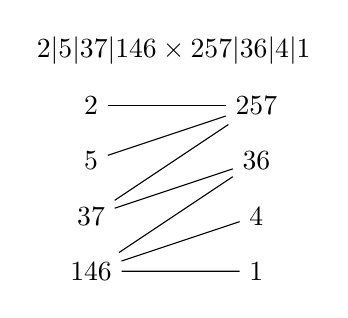
\begin{tikzpicture}[scale=.7]  
\node (p) at (0, 0) {$2|5|37|146 \times 257|36|4|1$};
\node (1) at (-1.5, -1) {$2$};
\node (2) at (-1.5, -2) {$5$};
\node (3) at (-1.5, -3) {$37$};
\node (4) at (-1.5, -4) {$146$};
%
\node (5) at (1.5, -1) {$257$};
\node (6) at (1.5, -2) {$36$};
\node (7) at (1.5, -3) {$4$};
\node (8) at (1.5, -4) {$1$};
%
\draw[-] (1)--(5); 
\draw[-] (2)--(5); 
\draw[-] (3)--(5); 
\draw[-] (3)--(6); 
\draw[-] (4)--(6); 
\draw[-] (4)--(7); 
\draw[-] (4)--(8);
%
\end{tikzpicture}
\caption{The strong complementary pair associated to the partition $2|5|7|3|6|4|1$.}
\label{fig:strong-complementary}
\end{figure}

There is a natural partial order on the facets of $\OP$. 
For two elements $x,y \in [n]$, we say that the set $\{x,y\}$ is an \emph{inversion} of a facet $(\sigma,\tau)$ if we have that $x<y$, the element $x$ appears before $y$ in $\sigma$, and the element $y$ appears before $x$ in $\tau$. 
%Visually, they appear as $\cdots | \cdots x \cdots | \cdots | \cdots y \cdots | \cdots$ in $\sigma$ and as $\cdots | \cdots y \cdots | \cdots | \cdots x \cdots | \cdots$ in $\tau$. 

\begin{definition}
    We say that two facets $(\sigma,\tau) \leq (\sigma',\tau')$ are comparable if the set of inversions of $(\sigma,\tau)$ is contained in the set of inversions of $(\sigma',\tau')$.
\end{definition}

It is immediate to see that this defines a poset.
\Guillaume{and even a lattice if a maximal and a minimal element are added?} 

\begin{proposition}
\label{p:crossings}
The set of inversions of a facet is in bijection with its set of edge crossings. 
Moreover, the set of facets with no crossings is the set of strong complementary pairs. 
\end{proposition}

\begin{proof}
    For the first part of the statement, it is clear that every inversion gives rise to a crossing. 
    For the converse, one needs to check that an anti-inversion, where $y$ appears before $x$ in $\sigma$ and $x$ appears before $y$ in $\tau$, cannot occur in a facet of $\OP$; this follows immediately from the $(I,J)$-conditions for $|I|=|J|=1$. 
    The second part of the statement follows from the fact that facets of the diagonal with no crossings are in bijection with permutations.
    As explained above, from a partition one obtains a strong complementary pair, which is in $\OP$. 
    In the other way around, given a strong complementary pair, one can read-off the partition in the associated tree, which has no crossings, by going along the edges from top to bottom, see \cref{fig:strong-complementary}.
\end{proof}


We aim now at characterizing the cover relations of this poset. 
Let $(\sigma,\tau)$ be a facet of $\OP$.
We say that a pair of adjacent blocks $\sigma_i | \sigma_{i+1}$ of $\sigma$ is \emph{admissible} if there is an element $\rho \in (\sigma_{i+1} \setminus \max\sigma_{i+1})$ such that $\rho < \min \sigma_{i}$ and $\rho < \min \gamma$ for $\gamma$ the unique path between $\sigma_i$ and $\sigma_{i+1}$. 
Such an element $\rho$ is said to be \emph{critical}. 
Let us define the \emph{left shift operator} $L$, which takes an admissible pair $\sigma_i | \sigma_{i+1}$ in $\sigma$ and creates a new ordered partition $L(\sigma)$ where the critical element $\rho$ is shifted one block to the left: we have $L(\sigma)_i := \sigma_i \cup \rho$, $L(\sigma)_{i+1} := \sigma_{i+1} \setminus \ \rho$, and $L(\sigma)_{j}:=\sigma_j$ for all $j\neq i, i+1$. 

In the same fashion, the \emph{right shift operator} $R$ sends an element $\rho \in (\tau_{i} \setminus \max\tau_{i})$ with $\rho < \min \tau_{i+1}$ and $\rho < \min \gamma$ one block to the right; the resulting ordered partition $R(\tau)$ is such that $R(\tau)_i := \tau_i \setminus \rho$ and $R(\tau)_{i+1} := \tau_{i+1} \cup \ \rho$.

\begin{definition}
    The facets of the \emph{dual SU diagonal} are the pairs or ordered partitions that can be obtained from an strong complementary pair $(\sigma,\tau)$ by iterated applications of the left shift operator $L$ on the first term $\sigma$, and iterated applications of the right shift operator $R$ on the second term $\tau$. 
\end{definition}

We shall show shortly that this definition recovers a dual of the SU diagonal on the permutahedra \cite{SaneblidzeUmble04}.

\begin{lemma}
\label{l:minima-invariance}
    Applying the left or right shift to a pair $(\sigma,\tau) \in \OP$ does not change the minima of the paths between adjacent vertices. 
\end{lemma}

\begin{proof}
We give the argument for the left shift, the one for the right one is similar. 
We observe that the paths in $(L(\sigma), \tau)$ are precisely the following: either they do not contain $\rho$, in which case they are paths of $(\sigma, \tau)$; or they do contain $\rho$, in which case they are obtained from paths in $(\sigma,\tau)$ by inserting at some place the unique path $\gamma$ between $\sigma_i$ and $\sigma_{i+1}$, or its inverse. 
Since $\rho < \min \gamma$, adding the path $\gamma$ does not change the minima of the paths in $(L(\sigma), \tau)$, with respect to the ones in $(\sigma, \tau)$.
\end{proof}

\begin{thm}
\label{t:iso-with-SU}
    The facets of the diagonal $\OP$ and the facets of the dual SU diagonal are equal. 
\end{thm}

\begin{proof}
Since we consider only the action of $L$ on the first term of the pair $(\sigma,\tau)$ and the action of $R$ on the second term, we will prove statements for $L$, the ones for $R$ are similar.

First we show that every facet of $\OP$ is a facet of the dual SU diagonal. 
Let $(\sigma,\tau)$ be a pair in $\OP$ and suppose that it satisfies the following property: for all pairs of consecutive blocks $\sigma_i | \sigma_{i+1}$ in $\sigma$, if $\min \sigma_i < \max \sigma_{i+1}$, then the unique path $\gamma$ between $\sigma_i$ and $\sigma_{i+1}$ has length $2$ and is given by $\{\min \sigma_i, \max \sigma_{i+1}\}$. 
In particular, we have $\min \sigma_i \geq \min \gamma$. 
We claim that $(\sigma,\tau)$ must be a strong complementary pair. 
To see this, suppose that $(\sigma,\tau)$ is \emph{not} a strong complementary pair; therefore by \cref{p:crossings} there exists an edge crossing. 
This implies that there is a minimal crossing, i.e. a crossing between edges adjacent to two consecutive blocks $\sigma_i | \sigma_{i+1}$. 
Since edges that are incident to a block are always in increasing order from bottom to top (this is a direct consequence of the $(I,J)$-conditions for $|I|=|J|=1$), there is a crossing between $\min \sigma_i$ and $\max \sigma_{i+1}$, which contradicts the property assumed above. 
So, there is no crossing in $(\sigma,\tau)$ and according to \cref{p:crossings}, we have that $(\sigma,\tau)$ is a strong complementary pair. 
The proof of the inclusion is now complete: if we are given a pair of facets $(\sigma,\tau)$ in $\OP$ which has at least one crossing, then there is a pair of consecutive blocks $\sigma_i | \sigma_{i+1}$ such that $\min \sigma_i < \max \sigma_{i+1}$ and $\min \sigma_i < \min \gamma$, and one can apply the inverse operator $L^{-1}$ shifting $\min \sigma_i$ to the right; and by induction we obtain a facet of the dual SU diagonal. 

Second, we show that every facet of the dual SU diagonal is in $\OP$. 
We already know that strong complementary pairs are in $\OP$. 
Thus, it suffices to prove that if a dual SU pair $(\sigma,\tau)$ is in $\OP$, then $(L(\sigma),\tau)$ is also in $\OP$. 
\cref{l:minima-invariance} shows that the minima of paths between consecutive vertices in $(L(\sigma),\tau)$ are the same as the ones in $(\sigma,\tau)$. 
Thus, all minima of paths in $(L(\sigma), \tau)$ are traversed from left to right, and we have $(L(\sigma), \tau) \in \OP$.
\end{proof}

\begin{proposition}
    \label{p:cover-relations}
    The cover relations of the poset of facets are precisely the pairs of the form $(\sigma,\tau) \prec (L(\sigma),\tau)$ and $(\sigma,\tau) \prec (\sigma,R(\tau))$ for some $L$ and $R$. 
\end{proposition}

\begin{proof} 
From the proof of \cref{t:iso-with-SU}, we know that for any facet $(\sigma,\tau) \in \OP$, we have that the pairs $(L(\sigma),\tau)$ and $(\sigma,R(\tau))$ are indeed facets of $\OP$. 

We show first that the left shift operator creates inversions, that is, for any $(\sigma, \tau) \in \OP$, we have that $(\sigma,\tau) \leq (L(\sigma),\tau)$. 
Observe that shifting a critical element to the left in $\sigma$ cannot delete any inversion: if $x<y$ and $x$ precedes $y$ in $\sigma$, then $x$ must precede $y$ also in $L(\sigma)$. 
Now, we need to show that for $x<y$, if either $y$ comes before $x$ in $\sigma$, or both $x$ and $y$ are in the same block of $\sigma$, then $y$ must come before $x$ in $\tau$. 
But this follows immediately from the $(I,J)$-condition for $I=\{x\}$ and $J=\{y\}$ defining $\OP$. 
The result then follows, since $\rho$ and $\max \sigma_{i+1}$ are in the same block of $\sigma$; thus $\max \sigma_{i+1}$ comes before $\rho$ in $\tau$ and the pair $(\rho,\max \sigma_{i+1})$ is an inversion of $(L(\sigma),\tau)$, which is not an inversion of $(\sigma,\tau)$. 

It remains to show that if $(\sigma,\tau) \leq (\sigma',\tau) \leq (L(\sigma),\tau)$, then we have either $\sigma=\sigma'$ or $\sigma'=L(\sigma)$. 
Indeed, if there is an inversion $(x,y)$ of $(L(\sigma),\tau)$ which is not an inversion of $(\sigma,\tau)$, then it must be that $x=\rho$. 
To the contrary, we have $\sigma=\sigma'$, which completes the proof. 
\end{proof}

Now we give the definition of the Saneblidze--Umble diagonal \cite{SaneblidzeUmble04}, following the description below Example $1$ in \cite{saneblidzeComparingDiagonalsAssociahedra2022}, and replace "$\max$" with "$\min$" and the symbol "$>$" with the symbol "$<$".

Let $(\sigma,\tau)$ be a pair of ordered partitions.
We say that a pair of adjacent blocks $\sigma_i | \sigma_{i+1}$ of $\sigma$ is \emph{SU admissible} if there is a non-empty subset $\rho \subset (\sigma_{i+1} \setminus \max\sigma_{i+1})$ such that $\max \rho < \min \sigma_{i}$. 
Let us define the \emph{subset left shift operator} $L^i$, which takes an SU admissible pair $\sigma_i | \sigma_{i+1}$ in $\sigma$ and creates a new ordered partition $L^i(\sigma)$ where the subset $\rho$ is shifted one block to the left: we have $L^i(\sigma)_i := \sigma_i \cup \rho$, $L^i(\sigma)_{i+1} := \sigma_{i+1} \setminus \ \rho$, and $L^i(\sigma)_{j}:=\sigma_j$ for all $j\neq i, i+1$. 
In the same fashion, the \emph{subset right shift operator} $R^i$ sends a subset $\rho \subset (\tau_{i} \setminus \max\tau_{i})$ with $\max \rho < \min \tau_{i+1}$ one block to the right; the resulting ordered partition $R^i(\tau)$ is such that $R^i(\tau)_i := \tau_i \setminus \rho$ and $R^i(\tau)_{i+1} := \tau_{i+1} \cup \ \rho$.


\begin{definition}[Dual SU diagonal, second definition]\label{def: Dual SU diagonal, second definition}
    The facets of the dual SU diagonal are the pairs of ordered partitions of the form $(L^{i_k}\cdots L^{i_1}(\sigma), R^{j_l}\cdots R^{j_1}(\tau))$ obtained from a strong complementary pair $(\sigma,\tau)$ by iterated application of subset left and right shifts operators, where moreover $i_1 > \cdots > i_k$ is decreasing and $j_1 < \cdots < j_l$ is increasing. 
\end{definition}

\begin{lemma}
\label{l:minima-invariance-subset}
    Applying the subset left or right shift to a pair $(\sigma,\tau)$ in the dual SU diagonal does not change the minima of the paths between adjacent vertices. 
\end{lemma}

\begin{proof}
    We analyse the left shift operator, the case of the right shift is similar. 
    First, we observe that any critical subset $\rho \subset L^{i_k}\cdots L^{i_1}(\sigma)_j, j \leq i_k$ satisfies $\max \rho < \min \gamma$, where $\gamma$ is the unique path between $L^{i_k}\cdots L^{i_1}(\sigma)_{j-1}=\sigma_{j-1}$ and $L^{i_k}\cdots L^{i_1}(\sigma)_j$. 
    Indeed, the path $\gamma$ is the same as the path between $\sigma_{j-1}$ and $\sigma_{j}$ in $(\sigma,\tau)$, and is equal to $\{\min \sigma_{j-1}, \max \sigma_j\}$; but since $\rho$ is critical we must have $\max \rho < \min \sigma_{j-1}=\min \gamma$. 
    The rest of the proof is the same as for \cref{l:minima-invariance}, with $\rho$ replaced by $\max \rho$. 
\end{proof}

\begin{proposition}
    The two definitions of the dual SU diagonal coincide. 
\end{proposition}

\begin{proof}
    We analyse the left shift operator, the case of the right shift is similar. 
    First, we observe that any subset left shift $L^{i}(\sigma)$ can be decomposed in a series of left shifts: since $\max \rho < \min \gamma$ by the proof of \cref{l:minima-invariance-subset}, we can first shift $\max \rho$ to the left, then $\max (\rho \setminus \max \rho)$, and so on until the entire subset $\rho$ has been shifted to the left. 
    This shows that any facet in the second definition of the dual SU diagonal is also a facet in the first definition. 

    For the reverse inclusion, we show by induction on the number of left shifts that a pair $(\sigma',\tau)$ where $\sigma'$ has been obtained by iterated left shifts can also be obtained by iterated subset left shifts, that is, can be written in the form $(L^{i_k}\cdots L^{i_1}(\sigma), \tau)$.
    The base case of a strong complementary pair is trivial. 
    Suppose that we are given a pair $(\sigma',\tau)$ where $\sigma'$ has been obtained by a sequence of $l+1$ left shifts. 
    By the induction hypothesis, the first $l$ left shifts can be rewritten as a sequence of subset left shifts, i.e. in the form $L^{i_k}\cdots L^{i_1}(\sigma)$ where $i_1 > \cdots > i_k$ are descreasing.
    Now suppose that the $(l+1)$-th left shift occurs between $L^{i_k}\cdots L^{i_1}(\sigma)_j$ and $L^{i_k}\cdots L^{i_1}(\sigma)_{j+1}$, with $j> i_k$ (otherwise, we are done!). 
    Let us denote by $\gamma$ the unique path between $L^{i_k}\cdots L^{i_1}(\sigma)_j$ and $L^{i_k}\cdots L^{i_1}(\sigma)_{j+1}$.
    By definition, we have that the critical element $\rho$ satisfies $\rho < \min \gamma$.  
    But by \cref{l:minima-invariance-subset}, this minimum is the same as the minimum of the path between $\sigma_j$ and $\sigma_{j+1}$, which is just $\min \sigma_j$. 
    Thus we have $\rho < \min \sigma_j$ (as well as $\rho < \min L^{i_k}\cdots L^{i_1}(\sigma)_j$, by criticality), and so $\rho$ can be integrated in a new or an existing subset left shift of the family $L^{i_k}\cdots L^{i_1}$, which completes the proof. 
    %also: maximum elements of each vertex never changes! so rho \neq max of its vertex
\end{proof}

One can thus interpret the left and right shift operators for singletons introduced by Saneblidze--Umble as generators of the poset of facets of the diagonal, with minimal elements the strong complementary pairs.

Now, we end with two important consequences of the preceding results. 
Consider the symmetry $s$ of the $(n-1)$-dimensional permutahedron, which consists in the reflection with respect to the hyperplane $x_1 + x_n = x_2 + x_{n-1}$. 
It sends an ordered partition $\sigma:=\sigma_1 | \ldots | \sigma_k$ to the ordered partition $s\sigma:=n-\sigma_{k}+1 | \ldots | n-\sigma_{1}+1$, where $n-\sigma_i+1$ is the set $\{n-j+1 \ | \ j \in \sigma_i\}$. 
\Kurt{This is what the next two corollaries should be i.e. altered to put max IJ =max J. Should probably combine with above.}
\begin{corollary}
\label{c:iso-with-SU}
The terms of the diagonal $\OP$ and the terms of the Saneblidze--Umble diagonal are in bijection through $(\sigma,\tau) \mapsto (s\tau,s\sigma)$
\end{corollary}

\begin{proof}
According to \cref{t:iso-with-SU}, it suffices to show that the symmetry $s$ sends the SU diagonal to the dual SU diagonal. 
\end{proof}

This allows us to prove a conjecture made in \cite[Remark 3.19]{LA21}.

\begin{corollary} \label{SU from hyperplane arrangement}
    The Saneblidze--Umble diagonal is given by the following choice of chambers in the fundamental hyperplane arrangement of the permutahedron: any vector $\vec v$ with strictly decreasing coordinates and which satisfy $\sum_{i \in I} v_i > \sum_{j \in J} v_j$ for all $I,J \subset \{1, \ldots, n\}$ such that $I \cap J = \emptyset, |I|=|J| \geq 2$ and $\max(I \cup J) \in J$ induces the Saneblidze--Umble diagonal on the $(n-1)$-dimensional standard permutahedron. 
\end{corollary}

\begin{proof}
    These orientation vectors are obtained precisely from the ones defining $\OP$ (see \cref{s:prelim}) via the symmetry described in \cref{c:iso-with-SU} above [...]. 
\end{proof}

This gives a geometric, alternative proof of the fact that all known diagonals of the associahedra agree \cite{saneblidzeComparingDiagonalsAssociahedra2022}.

\Guillaume{Thus, $(I,J)$-description for the SU diagonal...}

\Guillaume{Now we have matrix representation for free!}

\begin{example} \label{ex:shifts}
The permutation $5714632$ corresponds to the strong complementary pair $(\sigma,\tau) := 5|17|4|236 \times 57|146|3|2$. We now illustrate all possible shifts of this strong complimentary pair. The possible left shifts (indicated by their corresponding critical element, and drawn to avoid crossings) are
\begin{center}
\begin{tikzcd}
& 5|17|4|236 \times \tau \arrow[ld,"p=3"] \arrow[d,"p=1"] \arrow[rd,"p=2"]\\
5|17|34|26 \times \tau \arrow[rd,"p=1"] \arrow[d,"p=2"]&
15|7|4|236 \times \tau \arrow[rd,"p=2"] \arrow[d,"p=3"]&
5|17|24|36 \times \tau \arrow[d,"p=1"]\\
5|17|234|6 \times \tau \arrow[d,"p=1"]&
15|7|34|26 \times \tau \arrow[dl,"p=2"]&
15|17|24|36 \times \tau \\
15|7|234|6 \times \tau
\end{tikzcd}
\end{center}
The possible right shifts are simply
\begin{center}
\begin{tikzcd}
\sigma \times 57|146|3|2 \arrow[r,"p=1"] & \sigma \times 57|46|13|2 \arrow[r,"p=1"] & 57|46|3|12
\end{tikzcd}
\end{center}
As the left and right shifts can be performed independently we could combine these diagrams.
No other shifts are possible, observe for instance that we cannot perform the left shift $15|7|234|6 \times 57|46|13|2 \xrightarrow{p=2} 15|27|34|6 \times 57|46|13|2$ as the minimal path connecting $234$ and $7$ contains $1$ which is smaller than $2$ (see \cref{ex:ECbijection}). The unique way of producing $15|7|234|6 \times 57|146|3|2$ by the second definition of the SU diagonal \cref{def: Dual SU diagonal, second definition} is given by
\begin{center}
\begin{tikzcd}
5|17|4|236 \times 57|146|3|2 \arrow[r,"{p=\{2,3\}}"] & 5|17|234|6 \times 57|146|3|2 \arrow[r,"{p=\{1\}}"] & 15|7|234|6 \times 57|146|3|2
\end{tikzcd}
\end{center}
This corresponds to combining the top two arrows in the leftmost arrows of the diagram.
\end{example}



\subsection{Higher algebraic consequences}

\subsubsection{Shuffle trees}

\subsection{Topological enhancement}






